\documentclass[letterpaper,12pt,fleqn]{article}
\usepackage{matharticle}
\usepackage{pgfplots}
\usepackage{siunitx}
\pgfplotsset{compat=1.14}
\pagestyle{plain}
\begin{document}

\begin{center}
\Large Math-1003b Exam \#1
\end{center}

\vspace{0.5in}

Name: \rule{4in}{1pt}

\vspace{0.5in}

This exam is closed book and notes. You may use a scientific calculator;
however, no other electronics are allowed. Show all work; there is no credit
for guessed answers. All answers must be in factored form, where appropriate.
All numerical answers should be in exact values, unless you are specifically
asked for an approximate value.

\vspace{0.5in}

\begin{enumerate}
\item Perform the operation:
  \[\frac{y}{y^2-36}+\frac{2}{6-y}\]

  \vspace{2in}

\item Perform the operation:
  \[\frac{8(x-7)}{x^2+4x+4}\cdot\frac{2x+4}{4x-28}\]

  \newpage

\item Perform the operation:
  \[\frac{\frac{3-2y}{2y}}{\frac{3}{y}-2}\]

  \vspace{3in}

\item Solve for $w$:
  \[\frac{w}{5}-\frac{w+3}{w}=-\frac{3}{w}\]

  \newpage

\item Use the graph of $K(x)$ to answer the following questions:

  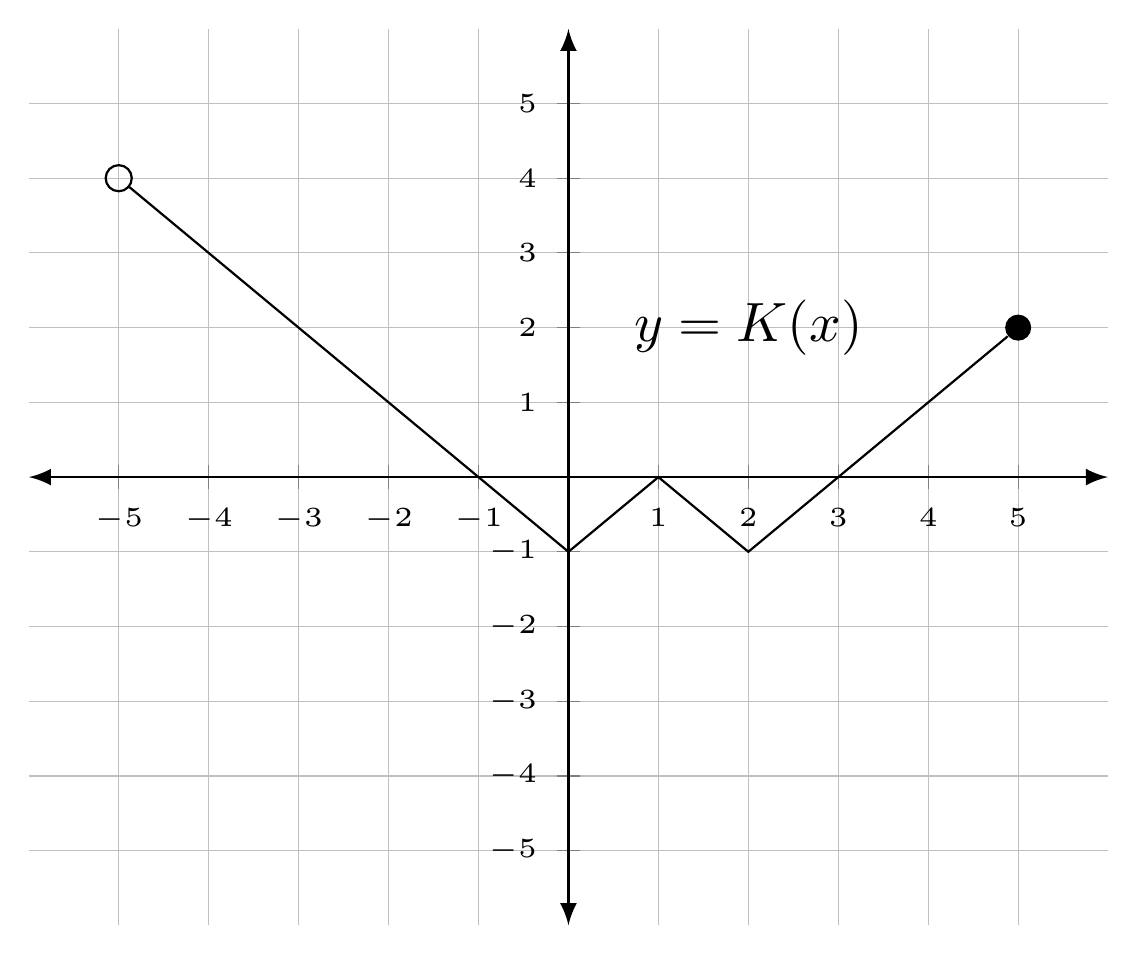
\begin{tikzpicture}[scale=2]
    \begin{axis}[
        xmin=-6,xmax=6,
        ymin=-6,ymax=6,
        grid=both,
        grid style={line width=.1pt, draw=gray!10},
        major grid style={line width=.2pt,draw=gray!50},
        axis lines=middle,
        axis line style={latex-latex},
        xtick={-5,-4,-3,-2,-1,0,1,2,3,4,5},
        ytick={-5,-4,-3,-2,-1,0,1,2,3,4,5},
        ticklabel style={font=\tiny},
      ]
      \node (a) [circle,draw,scale=0.5] at (-5,4) {};
      \node (b) [circle,fill,scale=0.5] at (5,2) {};
      \draw (a) to (0,-1) to (1,0) to (2,-1) to (b);
      \node at (2,2) {$y=K(x)$};
    \end{axis}
  \end{tikzpicture}

  \begin{enumerate}
  \item What is $K(2)$?

    \vspace{0.5in}

  \item What is the y-intercept?

    \vspace{0.5in}

  \item For what values of $x$ is $K(x)=0$?

    \vspace{0.5in}

  \item What is the domain of $K$, in interval notation?

    \vspace{0.5in}

  \item What is the range of $K$, in interval notation?
  \end{enumerate}

  \newpage
  
\item Given the function: $f(x)=2x-3$:
  \begin{enumerate}
  \item Is $f$ constant, linear, quadratic, or none of these?

    \vspace{0.5in}

  \item Find the y-intercept(s) of $f$.

    \vspace{1.0in}

  \item Find the x-intercepts(s) of $f$.

    \vspace{1.0in}

  \item Plot the intercepts of $f$ on the axes below and label the
    coordinates. Also draw the complete graph of $f$.
    
    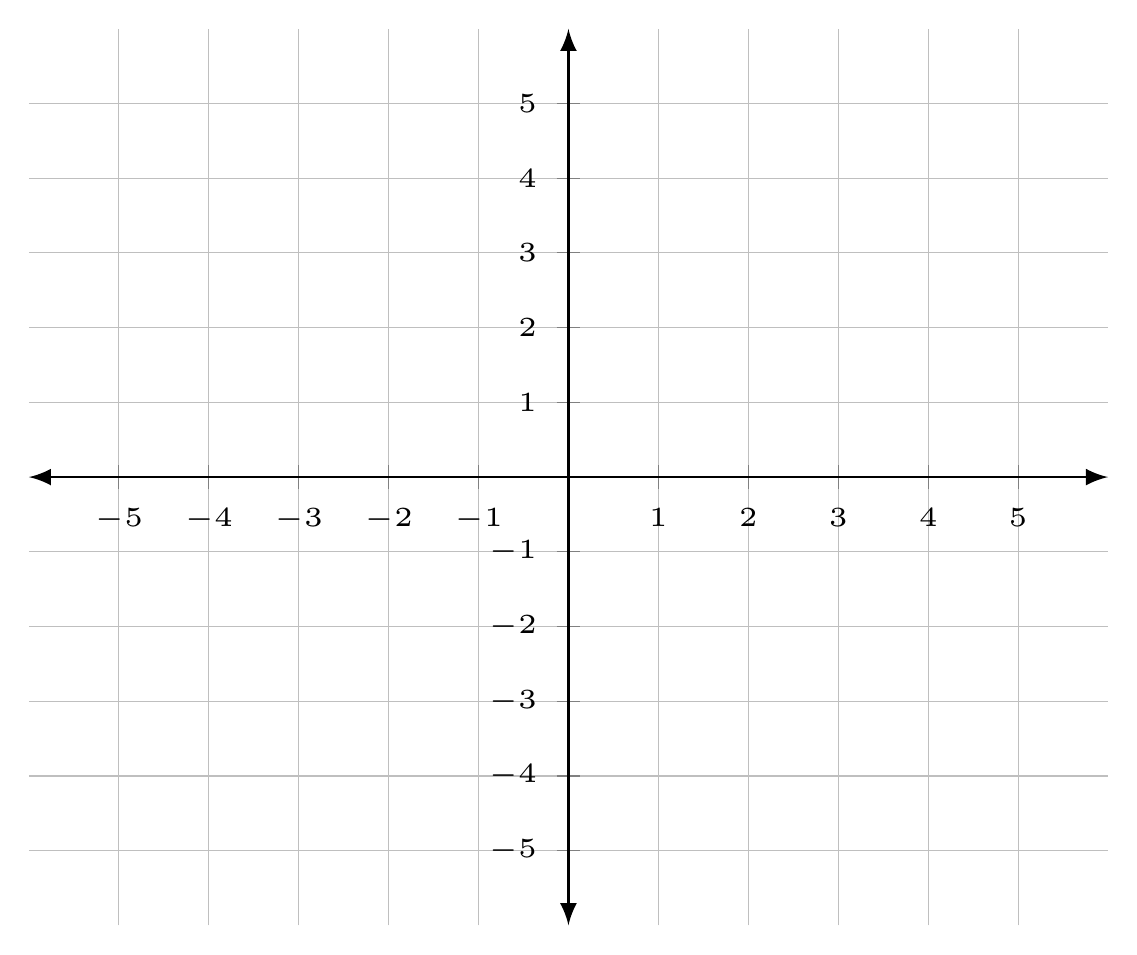
\begin{tikzpicture}[scale=2]
      \begin{axis}[
          xmin=-6,xmax=6,
          ymin=-6,ymax=6,
          grid=both,
          grid style={line width=.1pt, draw=gray!10},
          major grid style={line width=.2pt,draw=gray!50},
          axis lines=middle,
          axis line style={latex-latex},
          xtick={-5,-4,-3,-2,-1,0,1,2,3,4,5},
          ytick={-5,-4,-3,-2,-1,0,1,2,3,4,5},
          ticklabel style={font=\tiny},
        ]
    \end{axis}
  \end{tikzpicture}
  \end{enumerate}

  \newpage
  
\item David can run $\SI{2}{mph}$ faster that Rachel can run. David can run
  $\SI{15}{miles}$ in the same amount of time it takes Rachel to run
  $\SI{12}{miles}$. How fast can David and Rachel run?

\newpage

\item Given:
  \begin{eqnarray*}
    f(x) &=& x+3 \\
    g(x) &=& x^2+3x \\
    h(x) &=& x-2
  \end{eqnarray*}
  Do the following:
  \begin{enumerate}
  \item What is $(f-g)(x)$?

    \vspace{1.25in}
    
  \item What is $(g\circ f)(x)$?

    \vspace{1.25in}
    
  \item What is $(h\circ g)(1)$?

    \vspace{1.25in}
    
  \item What is $\left(\frac{f}{g}\right)(x)$?

    \vspace{1.25in}
    
  \item What is the domain of $\left(\frac{f}{g}\right)(x)$ in interval
    notation?
  \end{enumerate}

  \newpage

  \newcommand{\ans}{\rule{0.5in}{1pt}}

\item Match the following nine functions with the correct graph show below. Find
  the graph that matches each function and write the letter for that graph
  to the right of the corresponding function.

  \vspace{0.25in}

  \begin{minipage}[t]{3in}
    \begin{tabular}{lc}
      $f(x)=x$ & \ans \\
      \\
      $f(x)=x^2$ & \ans \\
      \\
      $f(x)=x^3$ & \ans \\
      \\
      $f(x)=\sqrt{x}$ & \ans \\
      \\
      $f(x)=\frac{1}{x}$ & \ans \\
    \end{tabular}
  \end{minipage}
  \begin{minipage}[t]{3in}
    \begin{tabular}{lc}
      $f(x)=\abs{x}$ & \ans \\
      \\
      $f(x)=2$ & \ans \\
      \\
      $f(x)=-x+1$ & \ans \\
      \\
      $f(x)=-x^2-x$ & \ans \\
    \end{tabular}
  \end{minipage}

  \vspace{0.25in}

  \begin{tabular}{ccc}
    \begin{tikzpicture}
      \draw [<->] (-2,0) -- (2,0);
      \draw [<->] (0,-2) -- (0,2);
      \draw [domain=0:2] plot (\x,{sqrt(\x)});
      \node at (-2,2) {$a)$};
    \end{tikzpicture} \hspace{0.25in} &
    \begin{tikzpicture}
      \draw [<->] (-2,0) -- (2,0);
      \draw [<->] (0,-2) -- (0,2);
      \draw [domain=0.5:1.9] plot (\x,{1/\x});
      \draw [domain=-1.9:-0.5] plot (\x,{1/\x});
      \node at (-2,2) {$b)$};
    \end{tikzpicture} \hspace{0.25in} &
    \begin{tikzpicture}
      \draw [<->] (-2,0) -- (2,0);
      \draw [<->] (0,-2) -- (0,2);
      \draw [domain=-1:2] plot (\x,{-(\x)+1});
      \node at (-2,2) {$c)$};
    \end{tikzpicture} \\
  \end{tabular}

  \begin{tabular}{ccc}
    \begin{tikzpicture}
      \draw [<->] (-2,0) -- (2,0);
      \draw [<->] (0,-2) -- (0,2);
      \draw [domain=-2:2] plot (\x,{(\x)});
      \node at (-2,2) {$d)$};
    \end{tikzpicture} \hspace{0.25in} &
    \begin{tikzpicture}
      \draw [<->] (-2,0) -- (2,0);
      \draw [<->] (0,-2) -- (0,2);
      \draw [domain=-2:2] plot (\x,{1});
      \node at (-2,2) {$e)$};
    \end{tikzpicture} \hspace{0.25in} &
    \begin{tikzpicture}
      \draw [<->] (-2,0) -- (2,0);
      \draw [<->] (0,-2) -- (0,2);
      \draw [domain=-1.4:1.4] plot (\x,{(\x)^2});
      \node at (-2,2) {$f)$};
    \end{tikzpicture} \\
  \end{tabular}

  \begin{tabular}{ccc}
    \begin{tikzpicture}
      \draw [<->] (-2,0) -- (2,0);
      \draw [<->] (0,-2) -- (0,2);
      \draw [domain=-1.25:1.25] plot (\x,{(\x)^3});
      \node at (-2,2) {$g)$};
    \end{tikzpicture} \hspace{0.25in} &
    \begin{tikzpicture}
      \draw [<->] (-2,0) -- (2,0);
      \draw [<->] (0,-2) -- (0,2);
      \draw [domain=-2:1] plot (\x,{-(\x)^2-(\x)});
      \node at (-2,2) {$h)$};
    \end{tikzpicture} \hspace{0.25in} &
    \begin{tikzpicture}
      \draw [<->] (-2,0) -- (2,0);
      \draw [<->] (0,-2) -- (0,2);
      \draw [domain=-2:2] plot (\x,{abs(\x)});
      \node at (-1,2) {$i)$};
    \end{tikzpicture} \\
  \end{tabular}

\end{enumerate}

\end{document}
